%Introduction
\chapter{Introduction}
According to the U.S. Department of Energy \cite{DOE2010} energy for heating and cooling accounts for approximately 35 - 45\% of the total expenditure within a building.  With such a large investment of energy being used to regulate the temperature of a building, any possible areas of improvement in this area are heavily sought after.  One idea for saving energy is to only regulate the temperature in rooms that are actually in use.  While the problem of determining what rooms are in use can be solved easily by a motion sensor, this problem becomes more difficult when the lead time to heat or cool a room is considered.  If accurate forecast models could be made for the occupancy of any section of the building, then a control scheme may be created that could save on total energy cost.

As another example where the forecasting of occupancy may be used to produce significant improvements, consider the roadways of the United States.  Optimal timing of traffic lights on major roadways across the United States could account for approximately a 22\% reduction in emissions along with a 10\% reduction in fuel consumption \cite{DOT2007}.  As of 2005 the total estimated fuel savings would amount to approximately 17 billions gallons of motor fuels annually.  If accurate estimates of future traffic patterns at each traffic light were available then dynamically changing the light timings to account for such traffic would improve overall traffic flow.

In both of the above scenarios motion through the environment can be captured through a network of many sensors.  For vehicular traffic systems, networks already exist using inductive loops and radar based sensors to count the number of cars in a given unit of time.  In the case of buildings, such networks are not as common.  To acquire such counts one could install a network using many infrared motion sensors and cameras to count human motion through the building.  

%Problem Statement
\section{Objective and Approach}
The objective of this work is to forecast the number of moving agents in a region of space $\delta$ seconds in the future.  This could be represented by a hypothesis function $h(x, \delta)$.  We will use mean absolute scale error (MASE) \cite{Hyndman2006} and mean absolute percentage error (MAPE) as  cost functions to compare with other previously implemented techniques.  Due to the level of noise present in traffic scenarios, the forecasted value of a sensor reading is aggregated for a time appropriate for the setting.  For vehicular traffic, most work deals with reading every 15 minutes to one hour.  For building traffic, this aggregation is 3 to 5 minutes.  

To assist in constructing models we make the assumption that data is generated from activities produced by human controlled entities moving through the environment.  Also we assume that the activities are repetitive and on some schedule.  The result of these assumptions is that from such scheduled movement we get sensors which have a spatial correlation and that for example, from week to week on the same day display similar trends.   Much of the research on traffic forecasting makes a similar assumption.  

We also assume that sufficient deviations from our forecasting function are often not the result of noise, but are due to an activity that does not commonly occur on that day.  Because such activities can overlap or occur at different times with varying amount of background noise present, it is a difficult task for one parametric model to accurately encapsulate all possible combinations of activities.  In an environment with many activities that could occur at multiple different times such combinations may be prevalent.  Past work doesn't address the problem of overlapping activities.  


\begin{wrapfigure}{r}{5cm}
\begin{center}
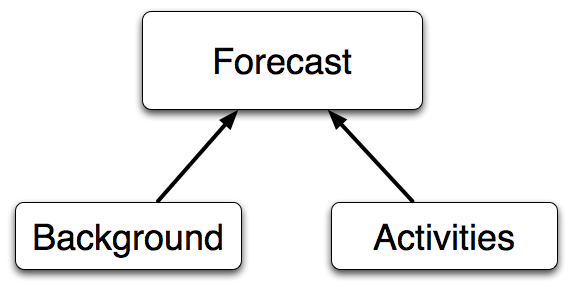
\includegraphics[width=0.30\textwidth]{flow_chart.png}
\end{center}
\caption{Forecasting is based on activities and a background model}
\label{fig:flow_chart}
\end{wrapfigure}

Our approach is to split the problem of forecasting into two parts: development of a background model and the development of a set of activity models.  Our background model is represented by a seasonal autoregressive integrated moving average (ARIMA) model.  To model activities, we propose comparing different models from activity recognition literature along with a new model which we propose here.  Forecasting is then performed using an ensemble predictor taking outputs from all trained activity models and the background seasonal ARIMA model.


%\section{Previous Work}
%Work in the past has attempted to solve this problem with parametric regression approaches such as fitting an auto regression moving average model (ARMA).  These models use a local history of forecasted values and actual readings to forecast future values.  The primary problem with these approaches is that due to being parametric with the background mean incorporated into the model, they tend to have problems with unusual patterns especially in the presence of changing means.

%There has also been a limited amount of work into using multiple models to predict future observations.  While such work has shown promise, there has also been a lack of research into discovery of the optimal timeframe and spatial influence of other sensors when considering such models.  Other predictive approaches tend to use the entire network.  We instead search for the best spatial features and temporal scales to perform prediction.


%Example Activity
\section{Example Activity}

\begin{figure}[ht]
\begin{center}
\subfloat[][Away game Sundays] {
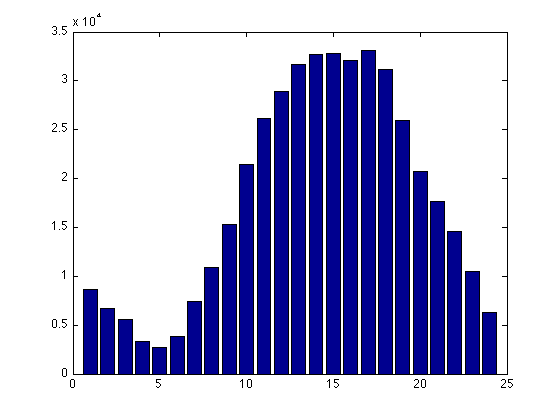
\includegraphics[width=0.45\textwidth]{broncos_off4.png}
\label{fig:broncos_off}
}
\subfloat[][Broncos game Sundays] {
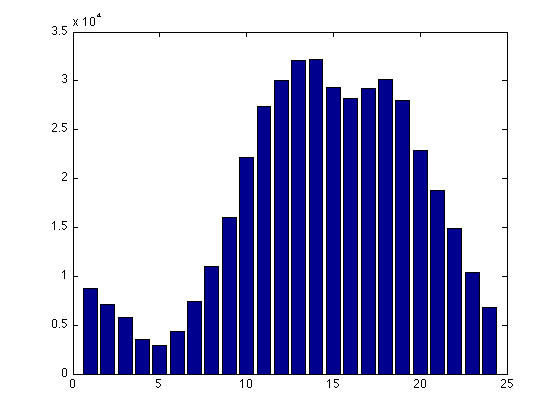
\includegraphics[width=0.45\textwidth]{broncos4.png}
\label{fig:broncos_on}
}
\end{center}
\caption{Total number of cars passing major highway sensors on Sundays in September and October 2010}
\label{fig:broncos}
\end{figure}

To illustrate an example of the need for our approach we provide the following example.  Figure~\ref{fig:broncos} shows the total counts of Denver traffic for each hour of the day averaged for the first four Sunday Broncos home games and for the first four Sunday away games in 2010.  Comparing figure~\ref{fig:broncos_off} with figure~\ref{fig:broncos_on} it is evident that a noticeable change in traffic patterns occur from approximately noon until approximately 6:00 pm.  This traffic change corresponds with a 2:05pm kickoff time for the game. 

Traditional parametric models have difficulty accounting for these different traffic patterns and the problem becomes more difficult when when it is considered that the Broncos may play a Sunday night game or a Monday night game.  To compound the problem further there may be multiple activities occurring at the same time such as a Rockies game and a Broncos game.  It is probable that the number of occurrences of such overlapping activities are few and that no training instances exist for traditional models to handle.  

Our approach will model each discrete activity separately and independent of the background model.  In this case a model for Broncos games and a model for Rockies games would be trained.  Once trained, accurate prediction should be possible despite the time of the games or the presence of other activities.

\section{Contributions}  
The contributions to the field of unsupervised traffic forecasting from this work are:
\begin{itemize}
\item{Use of activity models for improved forecasting accuracy of seasonal ARIMA models.}
%\item{A combined Bayesian prediction model which uses the results of a background model and activity models to predict future readings.}
\item{A new representation of activities using a mixture of time series multivariate Gaussians.}
\item{A new measure for determining activity model forecasting accuracy.}
\end{itemize}

\section{Structure of the Proposal}
The remainder of this proposal is outlined as follows.  Section two reviews current work related to traffic prediction and activity modeling.  Section three gives a summary of each dataset used in this work.  Section four details specific pieces of the overall approach.  All of the approach is not solved and where possible this section details potential ways to proceed with each unsolved part of the approach.  Finally section five is a time line of when the remaining work is expected to be completed.

